% Template PNSAC newsletter - Article
% Language: Latex
%

% Head

\title{My Days at the Home of the Merlin Engine}
\author{Richard Lodge}

\maketitle

I am a bean counter and I always wanted to be an engineer. For 5 plus
years in the late 1950s I had struggled to overcome the boredom of
training to be a Chartered Accountant in Leeds in Northern England. We
worked long hours for free because it was said that our bosses would
be giving us a valuable training.

\end{multicols}

\begin{figure*}[ht!]
   \vspace{2em}
   \centering
   %name of the graphic, without the path AND in EPS format:
   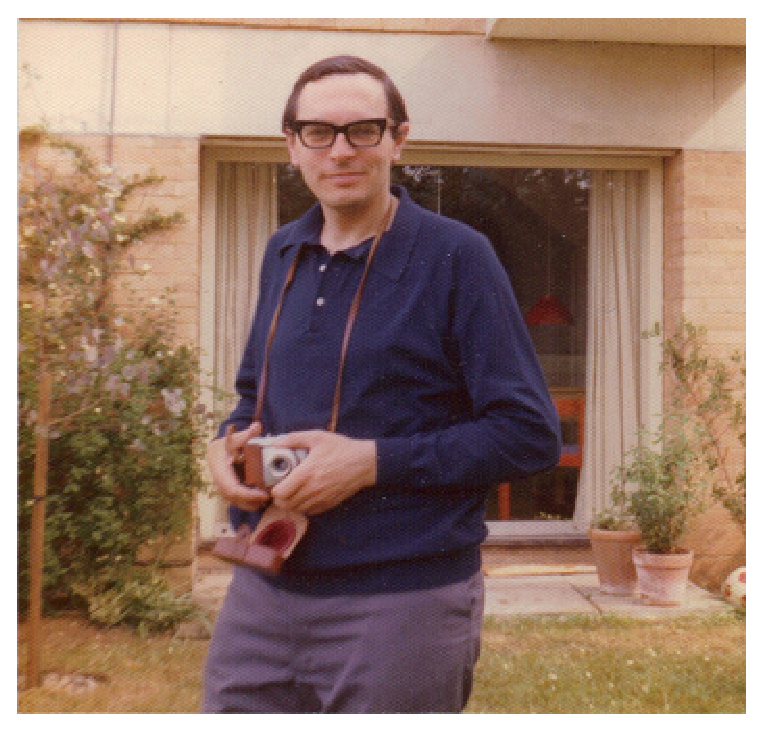
\includegraphics[scale=1.0]{richard_lodge.eps}
   %caption of the figure 
   \caption*{\small \em Richard Lodge in the 1970s.}
   %label of the figure, which has to correspond to \ref{}:
   \label{fig:richard}
\end{figure*}

\begin{multicols}{2}

Most of my friends were at university and enjoyed long summer holidays
when they would spend time tinkering with unreliable prewar old cars
while I toiled away in an office. Weekends were supposed to be spent
studying for accountancy exams. I always did the minimum amount of
study and would move into my father's big old garage at the earliest
opportunity to tinker with my 1934 Daimler limousine. The most common
tools I had to use were my hands, Whitworth spanners, feeler gauges, a
good sized hammer and Swarfega for cleaning up before doing a little
lightweight courting in the evenings.

Eventually the prized certificate arrived in the mail saying that I
had qualified as a Chartered Accountant. I was now ready to leave the
accountants' office behind and get a job as an accountant in
industry. I could hardly believe my luck when I was offered a job as
an assistant accountant in the Aero Engine Division of Rolls-Royce in
Derby.

\end{multicols}

\begin{figure*}[ht!]
   \vspace{2em}
   \centering
   %name of the graphic, without the path AND in EPS format:
   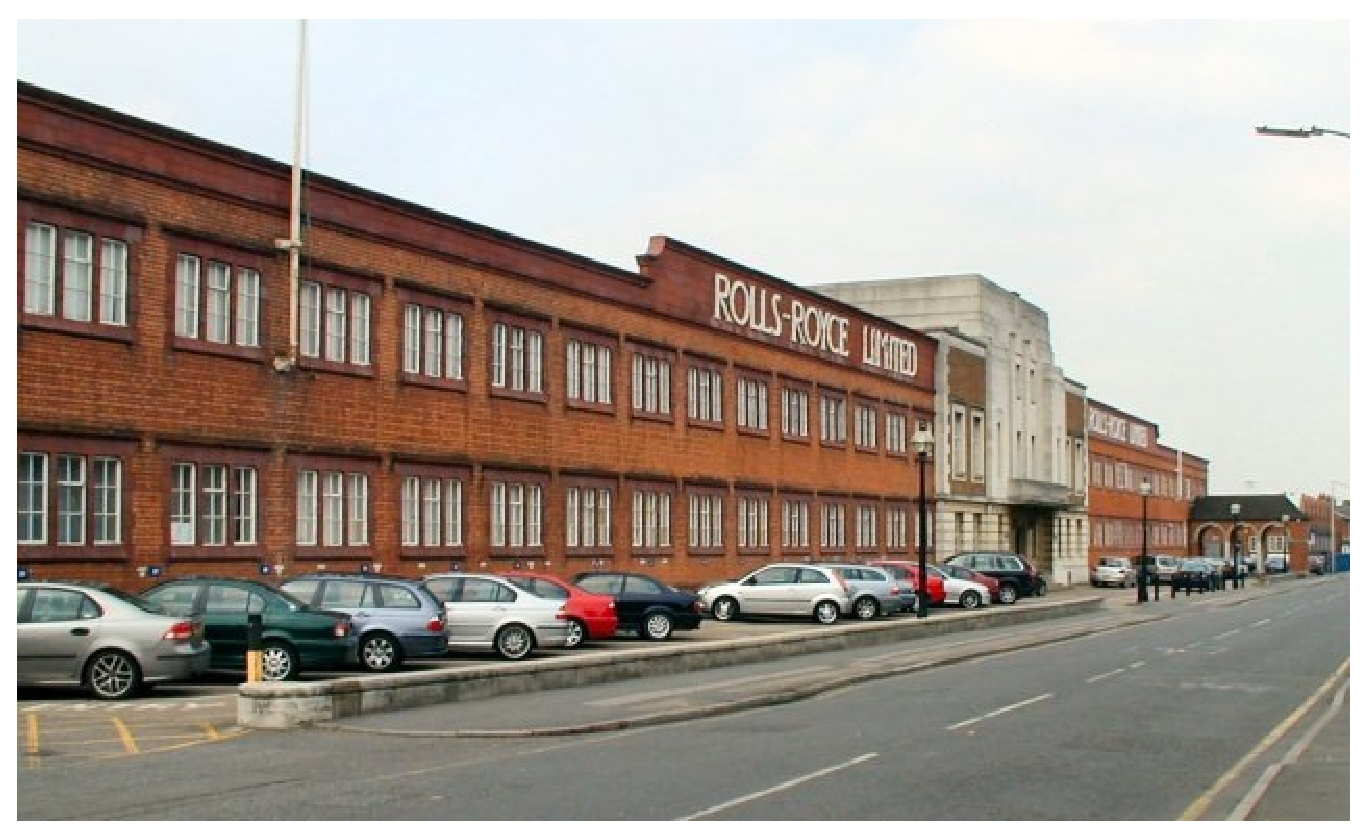
\includegraphics[scale=0.75]{rolls_royce.eps}
   %caption of the figure 
   \caption*{\small \em Nightingale Road office before closure in 2008.}
   %label of the figure, which has to correspond to \ref{}:
   \label{fig:rollsroyce}
\end{figure*}

\begin{multicols}{2}

As a young accountant I was very proud of myself to have got a job
with such a prestigious company and I duly reported to work on my
first Monday to be told that I would be given an induction period
under the guidance of an experienced employee. I found I was put with
two other green accountants to be guided by a man who was an ex WW2
regular army sergeant. He was about a foot shorter than me with a
pencil moustache but had a typical sergeant's voice and manner. Les
Hart knew very little about accounting and almost nothing about
engineering but he certainly knew the company and the world. One of
the best bits of advice he gave me was ``Do not let the buggers get you
down''. I needed this advice on many occasions while at Rolls-Royce.

Following a bewildering first week of being shown round some of the
R-R factories in Derby with my fellow new accountants, Les said we
were ready to start work. I was told to report to the Overheads
Department in the main accounting building near the Nightingale Road
head office. Les introduced me to the supervisor of the department and
then went on his way to deal with some other task. At that time R-R
employed about 30,000 people in several factories around the UK and I
felt very far removed from actual aero engines while sitting in this
vast sea of clerical people. The building was a converted warehouse
and my office was in the middle of the huge second floor housing about
200 people. There was no air conditioning and very little
ventilation. As the day wore on the atmosphere became putrid to say
the least of it. My pleasure at being offered a job at Rolls-Royce was
rapidly evaporating.

Derby in the 1960s was a two industry town, Rolls-Royce and the main
railway workshops of the Midland Region of British Railways. For many
people there were few choices other than to work at one of these two
employers. Many of the employees at R-R had been with the company
since leaving school at 16. They really did not like young
inexperienced accountants being foisted upon them but I was new, full
of enthusiasm and did not realize this.

The old sweats in the Overheads Department soon let me know that I
might be more technically qualified than them but that was only an
illusion. After a month or two, I made a bad mistake and my section
leader came to me and said ``You made a bad drop-off there''. I had no
idea what a drop-off was. He then called over the supervisor to
discuss the mistake and said ``Lodge here doesn't know what a drop-off
is and I guess he doesn't know whether he is punched, bored or
countersunk either.'' By that time I knew exactly what my mistake was
but what neither of these men explained was the meaning of their other
comments. It took me some time to find Les Hart who told me that a
drop-off referred to a careless person in the factory allowing an
expensive part to drop onto the floor and break and secondly that
punched, bored or countersunk described the method of making a certain
part of my anatomy. I was beginning to realize that to survive at R-R
I had a lot to learn.

Shortly afterwards I got my own back on these gentlemen when, to their
horror, I was appointed supervisor of the Overheads department.

In the next article I will describe how I came to enjoy the rest of my
time at R-R and learnt about life in the real world of traditional
British engineering.

\begin{footnotesize}
    \raggedleft PNSAC\\
\end{footnotesize}

% End of text.

%%% Local Variables: 
%%% mode: latex
%%% TeX-master: main_document.tex
%%% End: 

